\chapter{Angular Momentum}
\section{The Classical angular momentum}
Recall that the angular momentum for a system is given by :
\begin{equation}
\vec{L} = \sum_i \vec{ r}_i \wedge \vec{p}_i 
\end{equation}
With $ \wedge$ being the cross ( wedge) product between the position $\vec{r}_i$ and linear momentum $ \vec{p}_i$ of the $i$th degree of freedom in the system. For a single particle in 3 D we give a precise definition for the angular momentum :
\begin{equation}
\vec{L}= \begin{vmatrix}
\hat{x}& \hat{y} & \hat{z} \\ x& y & z \\ p_x & p_y& p_z
\end{vmatrix}
\end{equation}
\begin{figure}[h!]
	\centering
	\includegraphics*[scale=0.4]{./figures/ang}
	\caption{Illustration for the angular momentum of a classical rotating particle }
\end{figure}
\section{ Quantisation of the angular momentum}
One can apply the canonical quantisation for the angular momentum observable and turn in into a vector operator, since it is defined -classically- by the coordinates and linear momenta :
\begin{align}
[x^i, p_j]& = i\hbar \delta^i_j &  [x^i, x^j] =& 0 &  [ p_i ,p_j] &=0 
\end{align}
Hence the angular momentum operators are  ( dropping the hat) :
\begin{align}
L_x &= -i\hbar \left( y \partial_z - z\partial_y \right) \nonumber \\
L_y &= -i\hbar \left( z \partial_x - x\partial_z \right) \\
L_z &= -i\hbar \left( x \partial_y- y\partial_x\right) \nonumber 
\end{align}
Or we may write them in the spherical coordinates $(r, \varphi, \theta)$ :
\begin{align}
L_x &= i\hbar \left( \sin \varphi \partial_\theta + \cot \theta \cos \varphi \partial_\varphi \right) \nonumber \\
L_y &= i\hbar \left( -\cos \varphi \partial_\theta + \cot \theta  \sin \varphi \partial_\varphi \right) \\
L_z &= -i\hbar \partial_\varphi  \nonumber 
\end{align}
We also define the operator :
\begin{equation}
L^2 = L_x ^2+ L_y ^2+ L_z ^2
\end{equation}
It is a formidable, yet straightforward task to prove the following commutation relations:
\begin{subequations}
	\begin{align}
	[L_x,Ly]&=i\hbar L_z & [L_y,L_z]&= i\hbar L_x & [L_z,L_x]&=i\hbar L_y \\ [L^2, L_i]& =0 & \text{ For all} \;  i= x,y,z
	\end{align} 
\end{subequations}

We can also define the ( rising and lowering) operators:
\begin{equation}
L_\pm = L_x \pm i L_y
\end{equation}
Along with $L_z = L_3$ they satisfy a well-known commutation relations, known as the $su(2)$ algebra :
\begin{subequations}
	\begin{gather}
	[L_+,L_-] = 2 \hbar L_3 \\
	[ L_\pm, L_3] = \mp \hbar L_\pm 
	\end{gather}
	
\end{subequations}
The rising and lowering operators are expressed in the coordinate representation as :
\begin{equation}
L_\pm = \pm e^{\pm i \varphi}\left( \partial_\theta \pm i \cot \theta \partial_\varphi \right) 
\end{equation}
\section{The spherical harmonics }
As we maintain in the coordinate representation, we wonder about the eigenfunction for the operator $L_3$ and their properties. The operator $L_3$ has a special importance over the other two angular momentum operators, as the latter ones compose the ladder( rising and lowering) operators. We start by assuming such wavefunction :
\begin{eqnarray}
L_3 Y^{m} _ {\ell} ( \theta, \varphi) = m Y^{m}_{\ell} ( \theta, \varphi).
\end{eqnarray}
With $ m$ and $ \ell$ are eigenvalues, and $m$ takes an integer values between $ \ell$ and $ -\ell$, this shall be made clear in the next lecture. However, at the meantime, we just accept these as given facts.\\
Therefore, we conclude that :
\begin{equation}
Y^{m}_ {\ell} ( \theta, \varphi) = e^
{im\varphi} y _ { \ell m}
\end{equation}
Moreover,  the fact that$ L_\pm  y _ { \ell \pm \ell} =0$  gives us the differential equation:
\begin{equation}
\left( \partial_\theta - \ell \cot \theta \right) y _ { \ell \pm \ell} =0 
\end{equation}
Whose complete solution gives us the explicit expression of the functions $Y_{m} ^ {\ell}$, which are known as the \textbf{Spherical Harmonics }
\begin{equation}
Y^{m}_ {\ell} = (-1)^m \sqrt{\frac{2\ell+1}{4 \pi} \frac{(\ell+m)!}{(\ell-m)!}}e ^{im \varphi} P ^\ell _m (\theta)
\end{equation}
With $P ^\ell _m (\theta)$ is the associated Legendre Polynomial.\\
The spherical harmonics form a complete orthonormal basis for the Hilbert space :
\[
\mathcal{H} = \mathcal{L}^2 ( S^2, d\Omega)
\]
With $S^2$ being the unit sphere, and $ d\Omega = d \phi \sin\theta d\theta $, the solid angle element of the unit sphere. 
\section{Properties of the spherical harmonics }
\begin{itemize}
	\item Eigenvalue for $ L^2$ :
	\begin{equation}
	L^ 2 Y^{m} _ {\ell} ( \theta, \varphi) = \ell(\ell+1) Y^{m}_{\ell} ( \theta, \varphi).
	\end{equation}
	\item Orthonormality :
	\begin{equation}
	\int_{angles} Y^{m_1} _{\ell_1} ( \theta, \varphi) Y^{ *m_2} _ { \ell_2} ( \theta, \varphi) d\Omega = \delta_ {m_1,m_2}\delta_{\ell_1,\ell_2}
	\end{equation}
	\item Since the spherical harmonics form an orthonormal basis, the product of two of them is again expressed in terms of spherical harmonics. Take the product $ Y^{m_1}_ {\ell_1} ( \theta, \varphi)\cdot Y^{m_2} _{  \ell_2} ( \theta, \varphi)$, we can directly conclude that the resultant product is a multiple of the spherical harmonics having $M = m_1+m_2$ since the term containing $m$ is only an exponential, moreover, $L$ taking the range $ | \ell_1-\ell_2| \leq L \leq || \ell_1+\ell_2| $. The general rule for multiplication is given by Wigner $3j$-symbols ( or Clebsh-Gordon coefficients)  $C( \ell_1,m_1;\ell_2,m_2; L,M) $that shall be studied later in the addition of angular momenta. 
	\begin{align}
	Y^{m_1}_ {\ell_1} ( \theta, \varphi)\cdot Y^{m_2} _ {  \ell_2} ( \theta, \varphi) =& \sum _{M,L} \sqrt{\dfrac{(2\ell_1+1)(2\ell_2+1)(2L+1)}{4 \pi}} \nonumber \\
	&\qquad  \times \begin{pmatrix}
	\ell_1& \ell_2 & L \\ m_1 & m_2 &M
	\end{pmatrix} Y_{L} ^ {*M} ( \theta, \varphi) \begin{pmatrix}
	\ell_1& \ell_2 & L \\ 0 & 0 &0
	\end{pmatrix}
	\end{align}
	Where the Racah symbol is expressed in terms of $3j$ symbol
	\begin{equation}
	\begin{pmatrix}
	\ell_1& \ell_2 & L \\ m_1 & m_2 &M
	\end{pmatrix} = (-1)^{ \ell_1-\ell_2-M} \frac{1}{\sqrt{2L+1}} C( \ell_1,m_1;\ell_2,m_2; L,-M)
	\end{equation}
	These relations will prove useful as we discuss the addition of angular momenta.
	\item The Herglotz generating function \\
	If the quantum mechanical convention is adopted for the $Y_{\ell}^m$, then,
	\begin{equation}
	e^{v{\mathbf a}\cdot{\mathbf r}}
	= \sum_{\ell=0}^{\infty} \sum_{m = -\ell}^{\ell}
	\sqrt{\frac{4\pi}{2\ell +1}}
	\frac{r^{\ell} v^{\ell} {\lambda^m}}{\sqrt{(\ell +m)!(\ell-m)!}} Y_{\ell}^m.
	\end{equation}
	with
	\begin{equation}
	{\mathbf a}
	= {\mathbf{\hat z}}
	- \frac{\lambda}{2}({\mathbf{\hat x}} + i {\mathbf{\hat y}})
	+ \frac{1}{2\lambda}({\mathbf{\hat x}} - i {\mathbf{\hat y}})
	\end{equation}
	$\lambda$ here is a real parameter
\end{itemize}
More properties are found in the textbooks. We list here some of the spherical harmonics and their graphical representation:

\begin{align}
Y_{0}^{0}(\theta,\varphi)={1\over 2}\sqrt{1\over \pi}
\end{align}
\begin{align}
Y_{1}^{-1}(\theta,\varphi) &= & & {1\over 2}\sqrt{3\over 2\pi}\cdot e^{-i\varphi}\cdot\sin\theta & &= & &{1\over 2}\sqrt{3\over 2\pi} \cdot{(x-iy)\over r} \\
Y_{1}^{0}(\theta,\varphi)  &= & & {1\over 2}\sqrt{3\over  \pi}\cdot                   \cos\theta & &= & &{1\over 2}\sqrt{3\over  \pi} \cdot{z\over r} \\
Y_{1}^{1}(\theta,\varphi)  &= &-& {1\over 2}\sqrt{3\over 2\pi}\cdot e^{i\varphi}\cdot \sin\theta & &= &-&{1\over 2}\sqrt{3\over 2\pi} \cdot{(x+iy)\over r}
\end{align}

\begin{figure}[h!]
	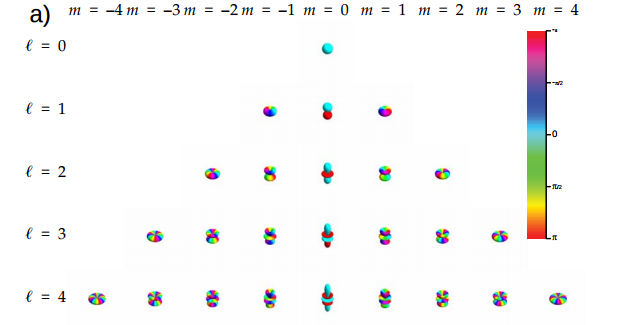
\includegraphics[scale=0.6]{./figures/spherical}
	\caption{Graphical representation for some of the spherical harmonics, the colour coding represents the probability density calculated via $|Y_{m} ^ {\ell} ( \theta, \varphi)|^2$}
\end{figure}
\section{Angular momentum eigenstates}
We now use more abstract method to analyse the angular momentum spectrum, by introducing the eigenstates for $L^2$ and $ L_3$
\begin{equation}
| \beta, m\rangle
\end{equation}
such that :
\begin{subequations}
	\begin{align}
	L^2 | \beta, m\rangle &= \beta  | \beta, m\rangle \\
	L_3 | \beta, m\rangle &= m \hbar | \beta, m\rangle.
	\end{align}
\end{subequations}
Now we look at the effect of the operators $L_\pm$ on the eigenstates:
\begin{align}
L_3 L_\pm | \beta, m\rangle &= L_\pm L_3 | \beta, m\rangle+ [ L_3,L_\pm]| \beta, m\rangle \nonumber\\
&=L_\pm ( L_3 \pm I) | \beta, m\rangle \nonumber \\
&= L_\pm (m \hbar \pm 1) \beta, m\rangle  \nonumber \\
\Rightarrow L_\pm | \beta, m\rangle &= | \beta , m\pm 1\rangle
\end{align}
Therefore, the operators $L_\pm$ acting on the eigenstates rise / lower the state, just like the creation and annihilation operators seen in the quantum harmonic oscillator. 
In fact, the operator $L_+$ rotates the angular momentum towards the $z$axis , whilst $L_-$ rotates it away from the $z$ axis towards the $-z$ axis.  
\begin{figure}
	\centering
	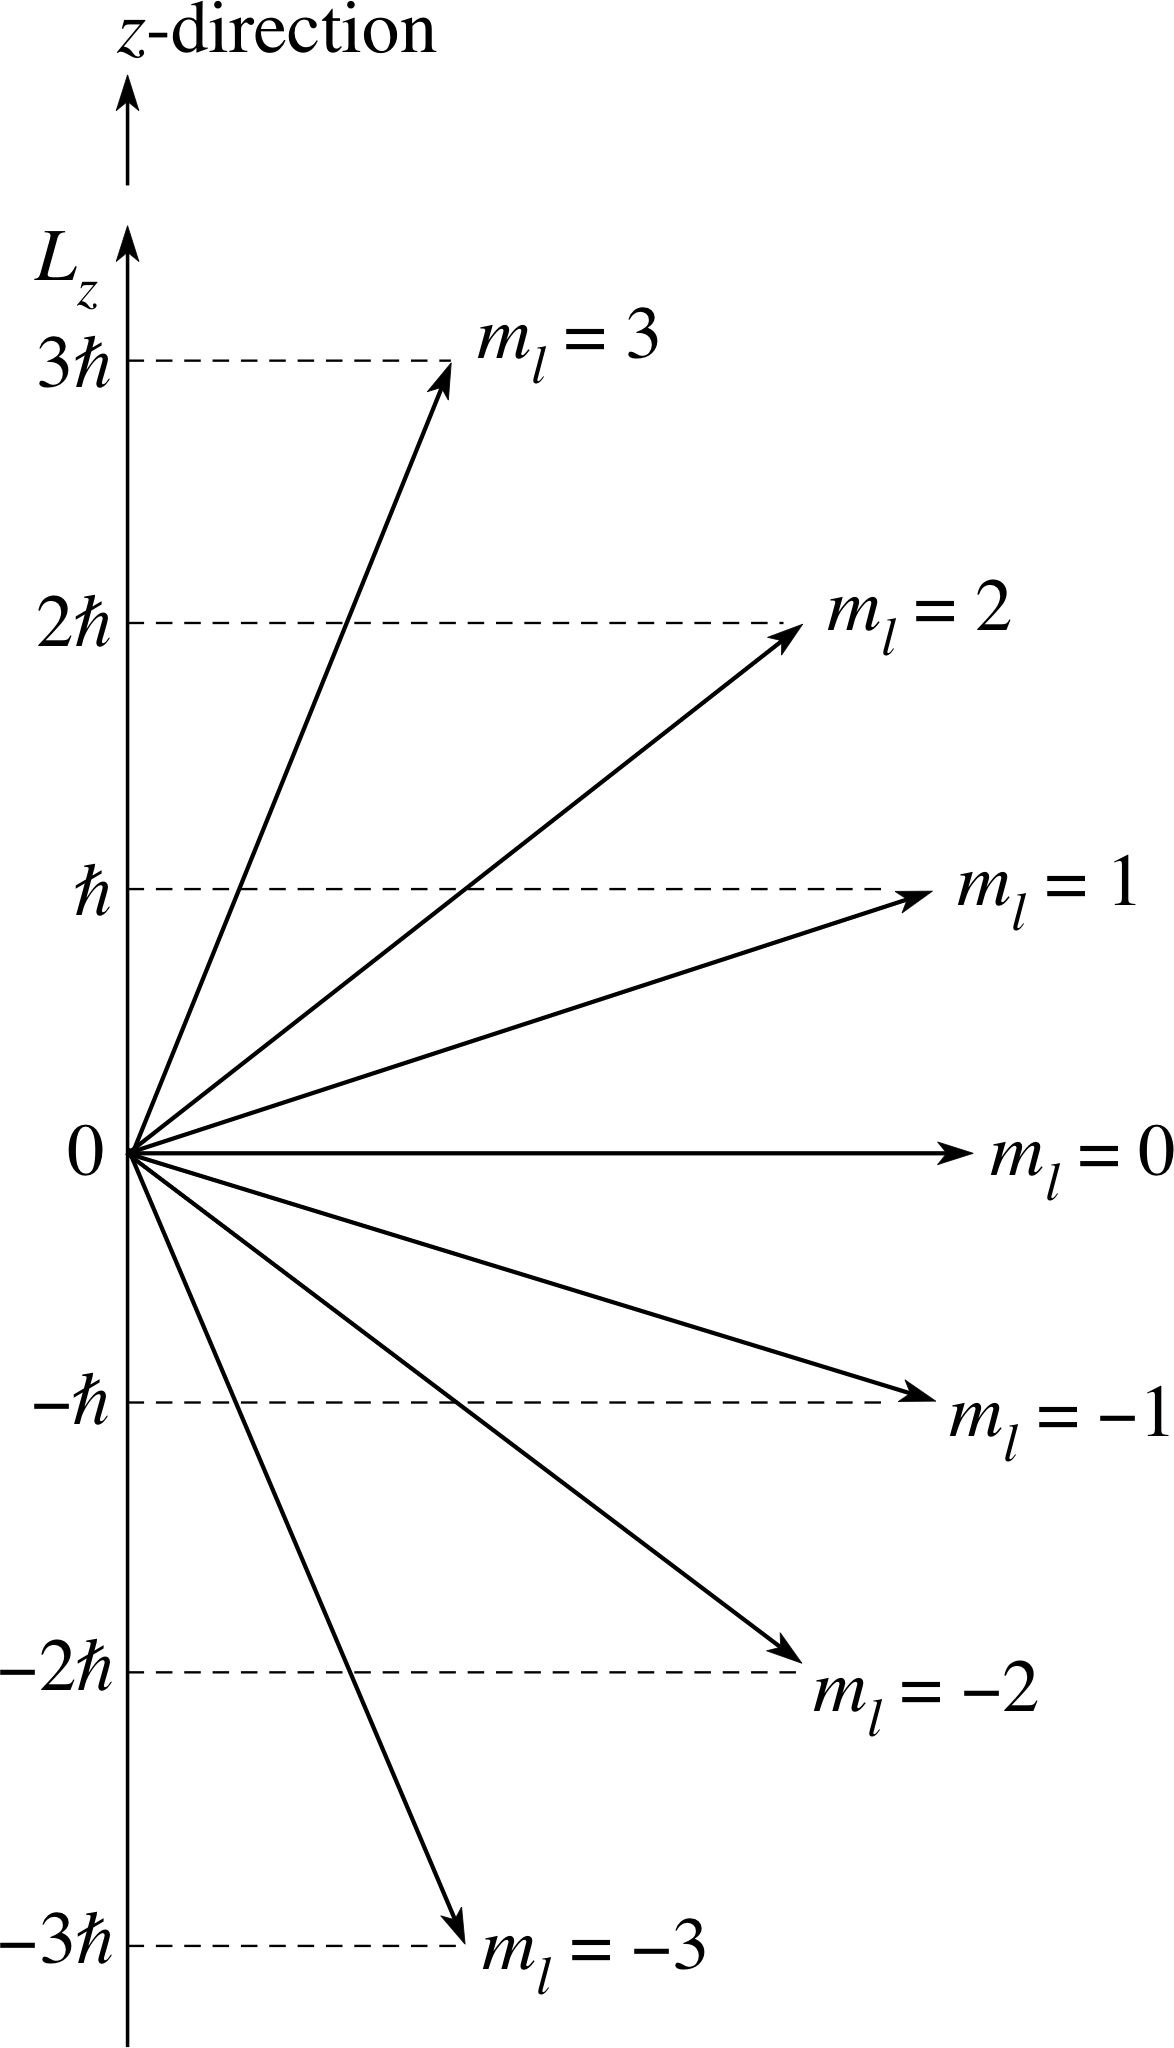
\includegraphics[scale=0.6]{./figures/z}
	\caption{The z-component of the angular momentum is quantised } 
\end{figure}
\section{The spectrum of angular momentum observable}
Now consider the following expected values :
\begin{subequations}
	\begin{align}
	\langle L _3 ^ 2\rangle &=  \hbar ^2 m^ 2 \\
	\langle L^ 2\rangle &= \langle L_1 ^ 2\rangle + \langle L_2 ^ 2\rangle+ \langle L_3 ^ 2\rangle \nonumber \\
	\beta 	&= a^2 +b^2 + \hbar ^2 m^ 2
	\end{align} 
	For some numbers $a$ and $b$.
\end{subequations}
In order to find the explicit relation between $\beta$ and $m$, we ought to investigate the spectrum of the angular momentum further. \\
We know, that for some value $m_{max}$ and $m_{min} $ : \begin{subequations}
	\begin{align}
	L_+ | \beta, m_{max}\rangle &= 0 \\
	L_-| \beta, m_{min}\rangle &= 0
	\end{align}
\end{subequations}
since the angular momentum will be totally alight with the wither $z$ or $z-$ after successive application of $L_+$ or $L_-$. If we let $\ell \hbar$ be the total angular momentum eigenvalue, then obviously $ m_{max} = \ell$ and $ m_{min} = - \ell$. \\
Now we analyse (5b) further :
\begin{align}
\langle\beta , m_{max }| L_+^ \dagger L_+ | \beta , m_{max} \rangle &= 0 \nonumber \\
\langle\beta , m_{max}| (L_1 -i L_2) 
(L_1+iL_2)  | \beta , m_{max} \rangle &= 0 \nonumber \\
\langle\beta , m_{max}| L_1^2 +L_2^2+i[L_1,L_2] | \beta , m_{max} \rangle &= 0 \nonumber \\
\langle\beta , m_{max}| L^2-L^2_3-L_3| \beta , m_{max} \rangle &= 0 \nonumber \\
\beta-\hbar^2m_{max}-\hbar m_{max}&=0 \nonumber \\
\Rightarrow \beta &= \hbar^2\ell(\ell+1)
\end{align}
Hence, we may denote the eigenstates in terms of $\ell$ instead of $\beta$, which is more physically relevant :
\[
| \beta,m \rangle \longleftrightarrow | \ell, m\rangle
\]
Such that:
\begin{equation}
L^2 | \ell, m\rangle = \hbar^ 2 \ell(\ell+1)
\end{equation}
Hence the magnitude of the angular momentum observable :
\begin{equation}
\langle L\rangle = \hbar\sqrt{\ell ( \ell+1)} 
\end{equation}
\begin{figure}[h!]
	\centering
	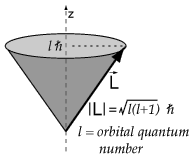
\includegraphics[scale=1]{./figures/z2}
	\caption{A vector model of the orbital quantum number  } 
\end{figure}
We may now write a full description for the angular momentum spectrum:
\begin{enumerate}
	\item The \textbf{orbital} angular momentum eigenvalue is $ \ell$, it refers to the maximum positive or negative value the orbital angular momentum can take.
	\item The z-component of the \textbf{orbital} angular momentum is $ m$ , sometimes , when other angular momenta are included we refer to it by $ m_\ell$ takes the \textbf{integer} values between $+ \ell$ and $ -\ell$.
	\item The length of the angular momentum is $ \hbar \sqrt{\ell(\ell+1)}$.
	\item We call $ \ell$ the orbital / azimuthal quantum number and $ m_\ell$ the magnetic quantum number. 
	\item There are other types of angular momenta, that shall be explored later, same analysis will be applied to them.
\end{enumerate}
\section{Problems}
\begin{enumerate}
	\item Verify that the operator $L^2$ commutes with all the angular momentum operator components $L_z,L_x$ and$ L_y$.
	\item Verify the commutator algebra relations for $L_\pm$ and $L_z$ using the commutator relations between angular momentum operator components commutation relations.
	\item Show that $ Y ^0_1$ and $Y^1_1$ are orthogonal. 
	\item Write the Hamiltonian operator for a system of two particles with reduced mass $\mu$ orbiting each other, in the position representation.
	\item Calculate directly the product $ Y ^1_1 \cdot Y ^0_1$.
	\item Write all the eigenstates for the orbital quantum number $ \ell = 3$ 
	\item Draw the $z$ components of the angular momentum states above
	\item What is the  minimal length of the momentum vector observable that carries the quantum number $ m= -4 \hbar$ ?
	\item What is $\ell$ for the free particle ? 
	\item Show that we can write $ \langle \varphi, \theta | | \ell, m\rangle$ as $ P_m( \varphi) F_\ell ( \theta)$ . 
\end{enumerate}